\documentclass[10pt]{article}

\usepackage{amsmath}
\usepackage{fullpage}
\usepackage{array}
\usepackage{graphicx}
\usepackage{gensymb}
\usepackage{booktabs}
\usepackage{gensymb}
\usepackage{graphicx}

\graphicspath{ {../Images/} }

\date{2014-6-22}
\pagestyle{empty}
\setlength{\parindent}{0pt}

\begin{document}
\begin{center}
\begin{Large}\textbf{Chapter: Frictional Force}\end{Large} \\
\smallskip
%\begin{large} Acceleration \end{large}
\end{center}
%%%%%%%
Objectives: Distinguish between static and kinetic friction, determine the direction and magnitude of frictional force.
\section{Frictional Force}
Definition: The tendency of a surface to oppose the \emph{relative} motion is called friction and the associated force is known as the frictional force. \\

\subsection{Origin of frictional force}
\begin{figure}[h]
\label{frictionsur}
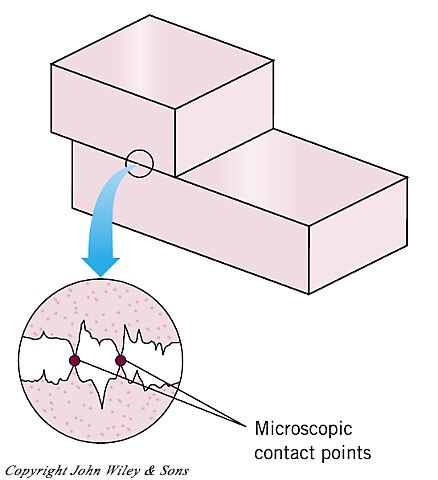
\includegraphics[scale=.8]{frictionsur}
\centering
\caption{Friction between surfaces}
\centering
\end{figure}
As shown in figure \ref{frictionsur}, the surfaces are highly irregular at the microscopic level.  The crests and trough of the surfaces get entangled with each other.  Therefore it requires additional force to overcome this friction between the surfaces and produce the relative motion.  

The coefficient of static/kinetic friction $\mu_{s/k}$ depends \textbf{only} on the nature of the surface.  Higher the irregularity of the surface, higher will be the coefficient of friction.

\subsection{Types of frictional force}
There are two types of frictional forces: 
\begin{enumerate}
\item Static friction is  the frictional force for body at rest.  The magnitude is given by
  \begin{equation}
    f_s=\mu_sN
  \end{equation}
where $N$ is the normal or contact force and $\mu_s$ is the coefficient of static friction.
\item Kinetic friction is the frictional force for body in motion. The magnitude is given by
  \begin{equation}
    f_k=\mu_kN
  \end{equation}
where $\mu_k$ is the coefficient of kinetic friction.
\end{enumerate}

In the figure \ref{skfriction}, the linear part corresponds to the static friction. It shows that the static frictional force is directly proportional to the applied force.  The latter part corresponds to the kinetic friction.

The maximum value of the static friction is always greater than the kinetic friction.  This implies that $\mu_s>\mu_k$

\subsection{An experiment on a book}
Consider a book kept on the table at rest.  Now we apply very small force parallel to the surface of the table.  The book doesn't move because there is a friction between the surface of the book and that of table which tends to oppose the relative motion.  We increase the magnitude of the applied force and the book still doesn't move.  This means that the frictional force also increased (why?). Now we apply force with even larger magnitude and then the book starts moving on the surface of the table.  There is still frictional force but it is smaller than the applied force.  The graph of this process is as following      
\begin{figure}[h]
\label{skfriction}
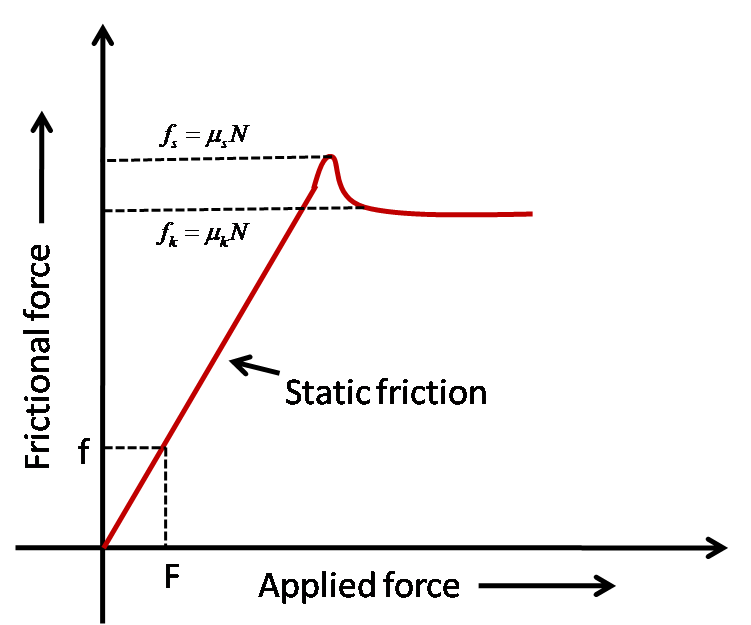
\includegraphics[scale=.5]{static_fric}
\centering
\caption{Frictional force vs applied force}
\centering
\end{figure}

\subsection{Sample Problems}
\begin{enumerate}
\item \begin{enumerate}
\item Find the direction and the magnitude of the frictional force in the setup shown in figure below.
\begin{figure}[h]
\label{qfric1g}
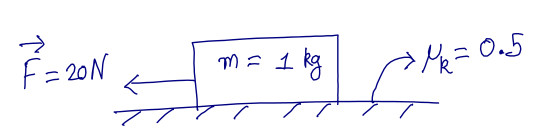
\includegraphics[scale=.5]{qfric1}
\centering
\end{figure}
\item Find the acceleration of the mass
\end{enumerate}
\item \begin{enumerate}
\item Find the direction and the magnitude of the frictional force in the setup shown in figure below.
\begin{figure}[h]
\label{qfric2g}
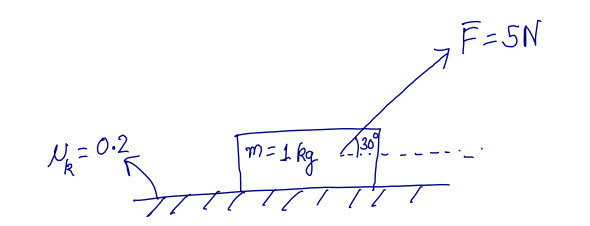
\includegraphics[scale=.5]{qfric2}
\centering
\end{figure}
\item Find the acceleration of the the mass
\end{enumerate}
\newpage
\item 
In the figure below, a 2.5 kg block is initially at rest on a horizontal surface.  A horizontal force $\vec{F}$ of magnitude 6.0 N and a vertical force $\vec{P}$ are then applied to the block.  The coefficients of friction for the block and surface are $\mu_s=.40$ and $\mu_k=.25$.  Determine the magnitude of the frictional force acting on the block if the magnitude of $\vec{P}$ is (a) 8.0 N, (b) 10 N, and (c) 12 N.  
\begin{figure}[h]
\label{qfric3g}
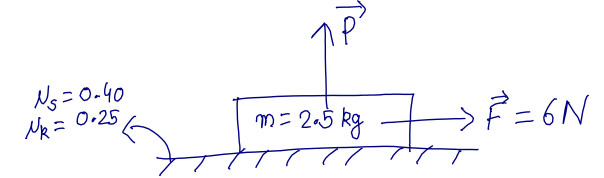
\includegraphics[scale=.5]{qfric3}
\centering
\end{figure}
\end{enumerate}

\end{document}
